\hspace{0.5cm} Our project contains the following tasks: 
\begin{itemize}
	\item Building and training the models required for Universal Style Transfer via Feature Transforms as described in \cite{bib11}.
	\item Implementing a PyTorch program to perform the UST algorithm as described in \cite{bib11}.
	\item Present innovative method to enhance the style transfer effect. This method shall be referred to as \textit{boosting}.
	\item In \cite{bib11}, Li et al present a method to transfer style from a pair of style images, in such a way that the result will contain stylistic aspects of both. Let's refer to this problem as \textit{Merge}-UST. In this task we research methods that utilize the UST framework to perform Merge-UST in a computationally lighter fashion than presented in \cite{bib11}.
\end{itemize}


\subsection{Models and Training}\label{subsec:Models}
\label{models_methods_lbl}
\hspace{0.5cm} In their paper \cite{bib11}, Li et al describe that in order to perform UST, the models required are five pairs of encoder-decoders based on the VGG-19 architecture. They work as a pipeline where each encoder-decoder pair is a pipeline level (see Fig.~\ref{fig:full-pipeline}). In each such pair, the encoder serve as feature extractor while the decoder does the inverse operation, reconstructs the image from the extracted features.\\
We based our solution on the implementation of VGG-19 \cite{bib20} in \texttt{torchvision.models}. It is trained for image classification on the ImageNet dataset (Deng et al.) \cite{bib21}. The model is available with pretrained weights. Its CNN feature extractor has the following architecture: 
\begin{gather*}
[64, 64, MP, 128, 128, MP, 256, 256, 256, 256, MP, 512, 512, 512, 512, MP, 512, 512, 512, 512, MP]
\end{gather*}

\subsubsection{Encoders}\label{subsec:Encoders}
Any numeric $d$ entry indicates a 2D-convolution layer with $d$ output channels, and MP entries indicate MaxPool layers. In order to build the five encoders, we load the \texttt{torchvision.models} VGG-19 pretrained model and trim it in the following way:
\begin{itemize}
	\item Encoder-1: [64]
	\item Encoder-2: [64, 64, MP, 128]
	\item Encoder-3: [64, 64, MP, 128, MP, 256]
	\item Encoder-4: [64, 64, MP, 128, MP, 256, 256, 256, 256, MP, 512]
	\item Encoder-5: [64, 64, MP, 128, MP, 256, 256, 256, 256, MP, 512, 512, 512, 512, MP, 512]
\end{itemize}
The encoders are initialized with pretrained weights and thus the project does not include encoder training. For next sections, denote Encoder-$j$ as $E_j$.

\subsubsection{Decoders}\label{subsec:Decoders}
The architecture of the decoders is generally inverse to that of the encoders, in order to achieve image-reconstruction. We defined five decoder \textit{blocks} the following way:
\begin{itemize}
	\item Decoder-Block-1: (64)[3]
	\item Decoder-Block-2: (128)[64, US, 64]
	\item Decoder-Block-3: (256)[128, US, 128]
	\item Decoder-Block-4: (512)[256, US, 256, 256, 256]
	\item Decoder-Block-5: (512)[512, US, 512, 512, 512]
\end{itemize}
The number in parenthesis in each row stands for the number of input channels for the block, and every US entry stands for an Up Sampling layer. Let's denote Decoder-Block-$j$ by $B_j$. Each decoder then is built as such:
\begin{equation}\label{eq:decoder}
D_j(x) = B_1 \circ \dots \circ B_j (x)
\end{equation}

Decoder training was done with two steps: Decoder-Block sequential training, followed by Fine-Tune phase.
\begin{itemize}
	\item \textbf{Decoder-Block sequential training}: Initially $B_1$ was trained to reconstruct images encoded by Encoder-1. Afterwards, each $B_j, j>1$ was trained once all $j-1,\dots,1$ had finished training to some reasonable degree. In training $B_j$, the reconstruction result for image $x$ was calculated by:
	\begin{gather*}
	\hat{x} = B_1 \circ \dots \circ B_{j-1} \circ B_j \circ E_j (x)
	\end{gather*}
	In this calculation all functions except $B_j$ are fixed. Since $B_{j-1}, \dots, B_1$ are already pretrained to some degree when training $B_j$, then $B_j$ learns to transform $E_j$'s output to $D_{j-1}$ input. The sequential blocks training is implemented in the \texttt{train\_block} function in \texttt{seq\_models.py} file. Use '\texttt{python seq\_models.py -h}' for help.
	
	\item \textbf{Fine-Tune Phase}: Each decoder $D_j$ is built according to Equation~\ref*{eq:decoder} with the pretrained blocks acquired in the previous step. With none of the blocks frozen, the entire $D_j$ is now trained for image reconstruction against $E_j$ and ultimately is saved as a decoder (and not as a bundle of blocks). The fine-tune training is implemented in the \texttt{train\_decoder} function in \texttt{models\_utils.py} file. Use '\texttt{python models\_utils.py -h}' for help.
\end{itemize}

Throughout this section, the loss function for training the models is:
\begin{equation}\label{eq:loss}
L = MSE(I_o-I_i) + \lambda \cdot MSE(\Phi(I_o)-\Phi(I_i))
\end{equation}
It is derived from Equation 1 at \cite{bib11}, with the difference that we use $MSE$ where Li et al use $L2 -loss$. We chose to use $MSE$ since different encoders $\Phi$ output different dimensions, causing the $L2$ loss to be  somewhat not as normalized as the $MSE$. For example, an input image $I_i$ of dimensions [3,1024,1024] would have features $f_4=E_4(I_i)$ of dimension [512, 128, 128] for $D_4$ training, 8,388,608 total entries, whereas it would have $f_5=E_5(I_i)$ of dimension [512, 64, 64] for $D_5$ training, 2,097,152 total entries. In this example, the dimension difference causes the feature loss to be much more important in $D_4$ training than in $D_5$ under $L2$, while we believe it shouldn't.

$\lambda$ was set to $1.0$ during training as advised by Li et al in their paper \cite{bib11}.

\textcolor{red}{TODO}: when training we encountered two problems: "boxy" artifacts in $D_4, D_5$ and border artifacts in $D_1$. to mitigate these problems we set the UpSampling in blocks 4,5 to "bilinear" whereas in 1,2,3 is "nearest", and in $D_1$ only, we set the padding method of $B_1$ from zero-padding to replicate padding.

\textcolor{red}{TODO}: discuss why we chose to train the models sequentially - smaller models converge faster, we wanted to use this to obtain a "good" starting point for the fine tuning.

\textcolor{red}{TODO}: COCO Dataset

\subsection{UST Algorithm}
\label{algo_methods_lbl}
The UST algorithm as described in \cite{bib11} formulates style transfer as an image reconstruction process coupled with feature transformation of whitening and coloring (WCT). The reconstruction step is responsible for inverting features back to the RGB space, the feature transformation step matches the feature statistics of a content image to a style image. The file \texttt{universal\_style\_transfer.py} implements the UST algorithm, use '\texttt{python universal\_style\_transfer.py -h}' for help.

\subsubsection{Architecture}
The basic building block of the UST is a pair of VGG based encoder and decoder, explained and described in ~\ref{models_methods_lbl}. A single level stylization pass in UST would be to pass a content image and a style image through an encoder, perform an transformation on the extracted content features called WCT, then reconstruct the output of the WCT using the decoder. The image output by the decoder should have both the original content and some notion of the artistic styles in the style image.\\ To achieve better results, UST does more than a single level stylization pass, it constructs a pipeline of such levels, each with its own encoder-decoder pair. Passing the content through this pipeline transfers style in different feature depths, so the result is generally more pleasing. See figure ~\ref{fig:full-pipeline} for a block diagram of the pipeline pass to perform UST on a pair of images $c,s$. In the following sections, for the $j$-th level of the pipeline denote the encoder by $E_j$ and the decoder by $D_j$.

\begin{figure}[h!]
	\centering
	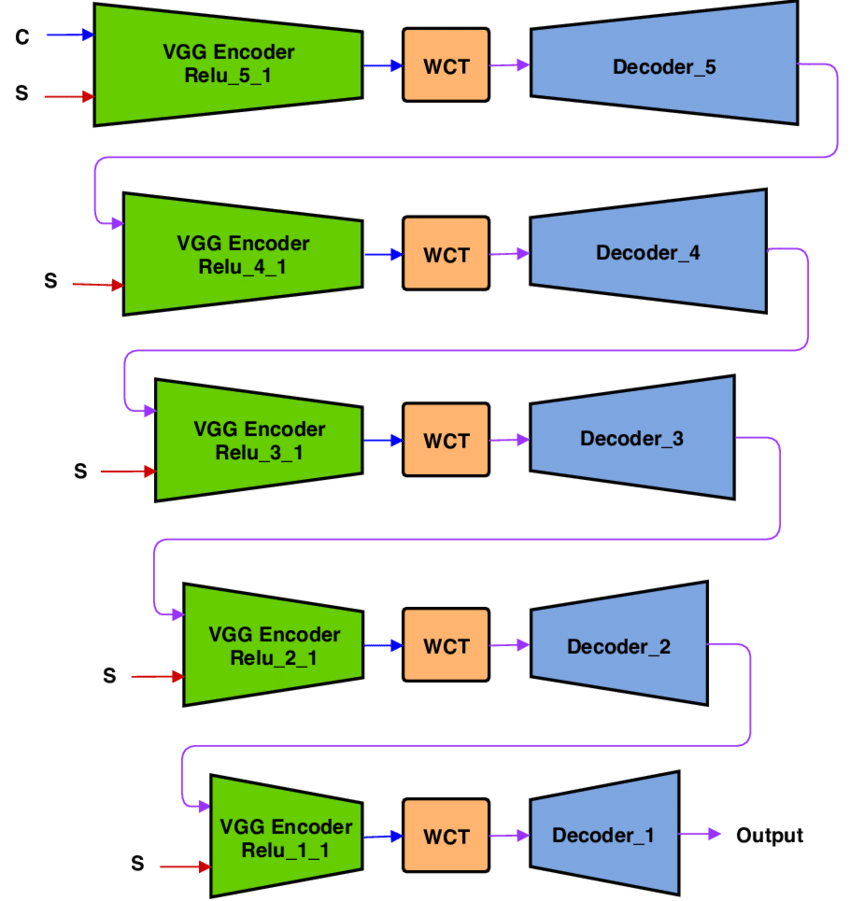
\includegraphics[width=0.5\linewidth]{UST_arc_mlt_level_pipeline.png}
	\caption{Universal Style Transfer pipeline architecture. Each level of stylization consists of single encoder-WCT-decoder network with different decreasing number of VGG layers. C and S are content and style images, respectively.
	}
	\label{fig:full-pipeline}
\end{figure}

\subsubsection{WCT} As explained above, given a pair of content image $I_C$ and style image $I_S$ as input for the $j$-th level, at first the encoder extracts their features by $f_c = E_j(I_C)$, $f_s = E_j(I_S)$. Notice that both these features are three dimensional, $f_c$ is $[c\times h \times w]$ and $f_s$ is $[c\times h' \times w']$. Their height and width are generally different but their number of channels, $c$, is the same.\\
The WCT is a pair of projection functions working on vectorized VGG features. The term \textit{vectorized} means that we treat every channel of the feature tensor as a row vector, so $\vec{f_c}$ is $[c \times hw]$ and $\vec{f_s}$ is $[c \times h'w']$. WCT works on the features extracted by the encoder, and its result is fed to the decoder, as seen in Figure ~\ref{fig:full-pipeline}. WCT is a composition of a whitening transform ($P_C$) and a coloring transform ($P_S$). The key idea behind the WCT is to directly match feature correlations of the content image to those of the style image via those two projections. Specifically, the WCT transform is applied to the vectorized content feature $\vec{f_c}$ via:
\begin{equation}
f_{cs} = P_S P_C \vec{f_c}
\end{equation}
Where $P_C=E_C\Lambda_C^{-\frac{1}{2}}$, and $P_S=E_S\Lambda_S^{\frac{1}{2}}$. Here $\Lambda_C$ and $\Lambda_S$ are the diagonal matrices with the eigenvalues of the covariance matrix $\vec{f_c} \vec{f_c}^T [c\times c]$ and $\vec{f_s} \vec{f_s}^T [c\times c]$ respectively. The matrices $E_C$ and $E_S$ are the corresponding orthonormal matrices of eigenvectors, respectively, (see figure ~\ref{fig:WCT-vis}). After the transformation, the correlations of transformed content features match those of the style, i.e., $\vec{f_{cs}} \vec{f_{cs}}^T = \vec{f_s} \vec{f_s}^T$.
The WCT performs well for artistic image stylization. However it generates
structural artifacts (e.g., distortions on object boundaries)
WCT is implemented in the function \texttt{wct} in file \texttt{utils.py}, \textcolor{red}{and explained in greater detain in section 3.2 in \cite{bib11}}.

\begin{figure}[h!]
	\centering
	\begin{subfigure}[b]{0.4\linewidth}
		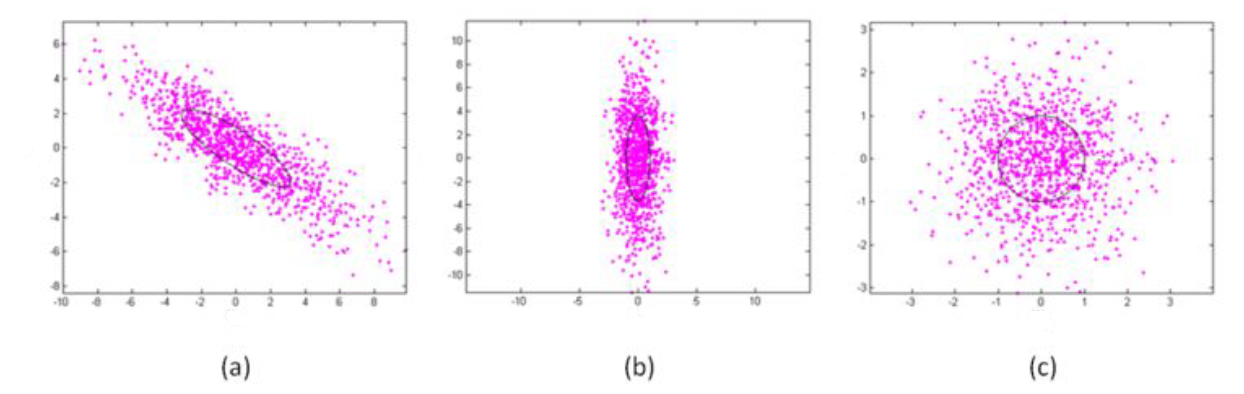
\includegraphics[width=\linewidth]{whitening.png}
		\caption{Data whitening}
	\end{subfigure}
	\begin{subfigure}[b]{0.4\linewidth}
		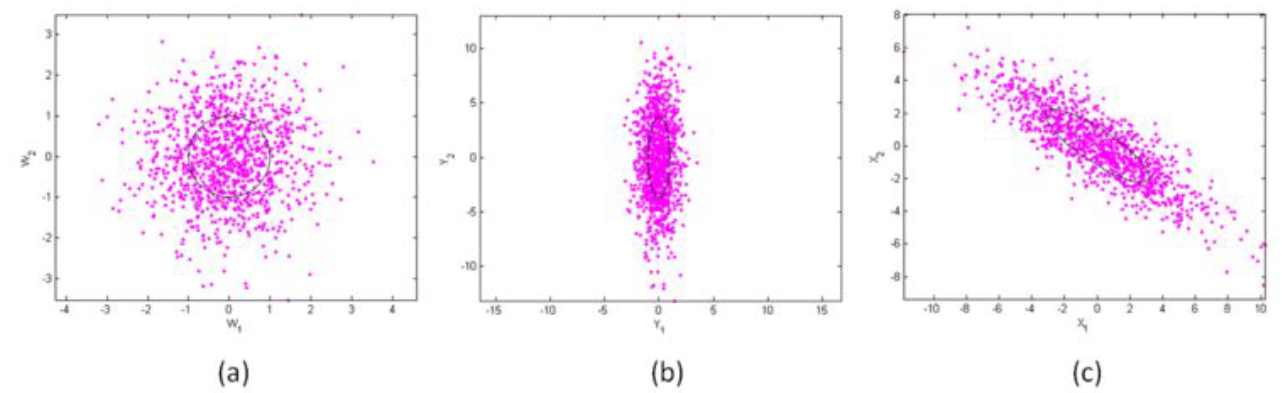
\includegraphics[width=\linewidth]{coloring.png}
		\caption{Data coloring}
	\end{subfigure}
	\caption{Whitening-Coloring-Transformation}
	\label{fig:WCT-vis}
\end{figure}

\subsection{Boost}
\label{boost_methods_lbl}
The Boost step is a fruit of our invention, and it enhances the effect of style transferral of the UST in selected regions of the image. The motivation for this \textbf{boosting} method comes from the desire to better utilize the capability to perform a constant number of SVD calls on matrices as big as $[512\times 512]$ without slowing down UST considerably. The time complexity of SVD is $O(n^3)$ for square matrices, so we treat 512 as the upper bound on the size of matrices we want to call SVD on. Empirically, SVD works in reasonable time on square matrices up to the upper bound, but we expect the its runtime to grow very rapidly for larger matrices. In the pipeline described in Figure ~\ref{fig:full-pipeline}, levels 1 and 2 use $E_5, E_4$ respectively to extract a 512-channels feature map representation of $I_c$ and $I_s$. This leads the WCT procedure to make two SVD calls on $[512\times 512]$ matrices, as described in ~\ref{subsec:arch}. We consider these calls \textit{efficient}. On the contrary, in levels 3,4,5, the encoders extract feature maps with 256, 128 and 64 channels respectively. These calls are \textit{inefficient} since they call SVD on matrices of size lower than the upper bound.\\

The \textit{Boost} step is a procedure done after the WCT had output $f_{cs}$ and before image reconstruction took place, in levels of the pipeline where there are inefficient SVD calls, i.e. in architectures 1, 2 and 3. At encoder-decoder architecture $j\in\{1,2,3\}$, let $x$ be the input content, $f_c = E_j(x)$ be the content features of dimensions $[c \times h \times w]$, and $f_s = E_j(s)$ be the style image features of dimensions $[c \times h' \times w']$. The number of channels $c$ is either 64, 128 or 256. The \textit{Boost} step consists of the following sub-steps:
\begin{enumerate}
	\item This sub-step will synthetically create $f_c^b$ and $f_s^b$ of 512 channels with reduced height and width, such that the total number of entries in $f_c$ is the same as in $f_c^b$ and likewise for $f_s$ and $f_s^b$. Maintaining tensor sizes is important since many times regular UST is working close to the GPU memory limit also without boosting, so we wouldn't wish to create tensors much larger than we already handle. For architecture-1, $c=64$. Choose 8 rectangular regions of size $[c \times h/4 \times w/2]$ from $f_c$ and 8 rectangular regions of size $[c \times h'/4 \times w'/2]$ from $f_s$. The regions are to be stacked on the channel dimension to achieve $f_c^b$ of size $[8c \times h/4 \times w/2]$ and $f_s^b$ of size $[8c \times h'/4 \times w'/2]$. Notice that $8c=512$ as desired. Similarly for architecture-2, choose 4 regions while dividing both height and width by factor of 2. For architecture-3 choose 2 regions while dividing height by 2, width is not divided in this case. Parts (a), (b) and (c) in Figure ~\ref{fig:boost} depict this sub-step. 
	
	\item Call the WCT procedure on $f_c^b$ and $f_s^b$ to obtain $f_{cs}^b$. Since both $f_c^b$ and $f_s^b$ have 512 channels, the two SVD calls in the WCT decompose $[512\times 512]$ matrices. Depicted in part (d) of Figure ~\ref{fig:boost}.
	
	\item Next, split $f_{cs}^b$ across the channel dimension to invert the stacking operation done previously. Let these splits be $r_1^b, \dots r_d^b$ where $d\in\{2,4,8\}$ depending on the architecture. These splits are now being treated as boosted style transformed regions of $f_{cs}$. For architecture-1 we get 8 such regions, for arch-2 we get 4 and for arch-3 we get 2.
	
	\item Lastly, blend these regions with $f_{cs}$. Let $R_i$ be the indices slicing region $i$ from $f_c$, i.e. $f_c[R_i]$ is the $i$-th region, then:
	\begin{equation}
	f_{cs}[R_i] = (1-k)\cdot f_{cs}[R_i] + k\cdot r_i
	\end{equation}
	$k$ is a kernel the size of the regions $r_i$ that diminishes close to its exterior. Its purpose is to blend $r_i$ into $f_{cs}[R_i]$ with no visible border artifacts. For $k$ we used a 2D raised-cosine which answers this requirement. See implementation in \texttt{raised\_cosine\_kern} function in \texttt{utils.py} file. The last two sub-steps are depicted in part (e) of Figure ~\ref{fig:boost}.
\end{enumerate}
The boost step is implemented in \texttt{boost} function in \texttt{utils.py}.\\

\begin{figure}[h!]
	\centering
	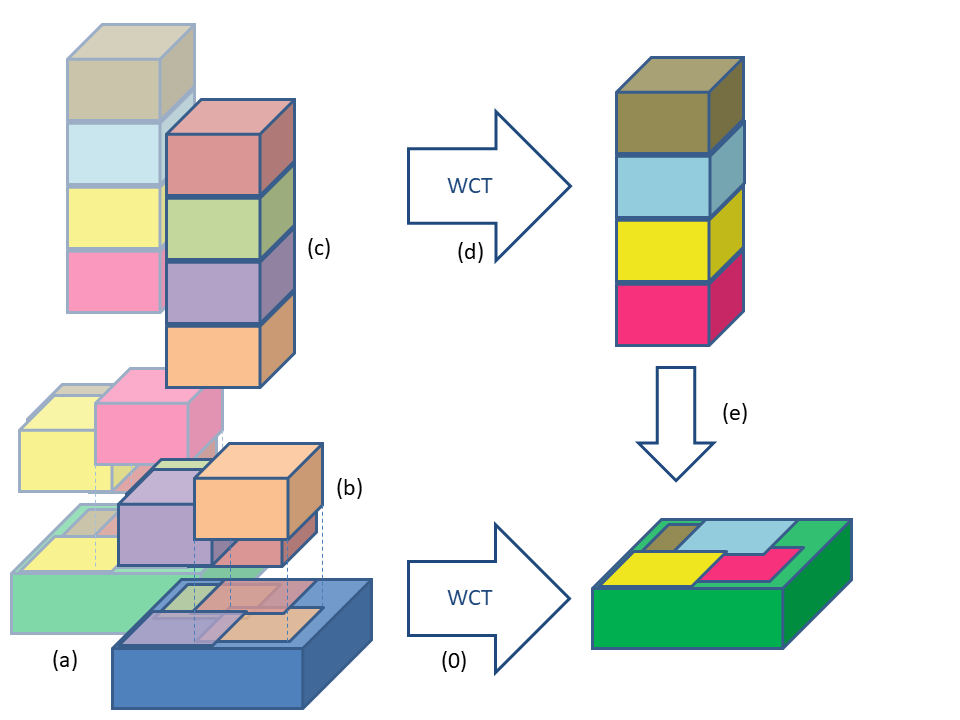
\includegraphics[width=0.6\linewidth]{boost_fig.png}
	\caption{Boost main steps. (0) is the ordinary WCT on $f_c$ and $f_s$, (a) is regions selection, (b) is region slicing, in (c) the regions are stacked, in (d) WCT is performed on the stacked regions with 512 channels, finally in (e) the boosted regions are blended into $f_{cs}$.}
	\label{fig:boost}
\end{figure}

Before refining the boost method to its final form we had tried to replace the original WCT altogether in architectures 1,2 and 3, such that \textbf{only} efficient SVD calls are conducted. Doing so, regions were not chosen, instead, the features were perfectly split into non overlapping sections. These were stacked, then came WCT, after which the sections were unstacked. The major drawback of that method is that these sections are treated as independent channels in the WCT, so clear border artifacts could be seen between them after the reconstruction. 



\subsection{Merge}
\label{merge_methods_lbl}
In their paper \cite{bib11}, Li et al describe an interpolation technique to generate texture from two input style images. According to their method, which we shall refer to as \textit{Original-Merge}, at each pipeline level two WCT calls are conducted: $f_{cs_1} = WCT(x, f_{s_1}), f_{cs_2} = WCT(x, f_{s_2})$ where $x$ is the content features output by the level encoder. The results are then interpolated with $f_{cs} = \beta f_{cs_1} + (1-\beta)f_{cs_2}$. After the interpolation, $f_{cs}$ is reconstructed as usual using the level decoder.\\

In this section we researched other merging techniques to merge two style with a \textbf{single} WCT call for each pipeline level. We present the following three techniques:

\begin{itemize}
	\item \textbf{Level Merge}: Let $P_1, \dots, P_k$ be the pipeline level functions. According to this notation, in Figure ~\ref{fig:full-pipeline} the output is a product of:
	\begin{equation*}
	I_{out} = P_5 ( P_4 ( P_3 ( P_2 ( P_1 (c,s),s) ,s),s), s)
	\end{equation*}
	To \textit{Level Merge} transfer content $c$ with style images $s_1$ and $s_2$ do the following:
	\begin{equation*}
	I_{out} = P_5 ( P_4 ( P_3 ( P_2 ( P_1 (c, s_1), s_2), s_1), s_2), s_1)
	\end{equation*}
	This method simply alternates the transferred style at each progression through the pipeline levels. In Level-Merge, the WCT procedure is called once per level, which makes it more computationally efficient than Original-Merge. Since in each level it calls for the encoder twice, the WCT once, and the decoder once, it has the same computational load of regular UST with one style image. As a side note, the $\beta$ parameter that controls the relative weight of each style cannot be used in this technique.
	 
	\item \textbf{Channel Merge}: Let $s_1, s_2$ be the input pair of styles, and let $c'$ be the content input to the $j$-th pipeline level. Under Channel Merge, we extract features for all three: $f_{s_1} = E_j(s_1), f_{s_2} = E_j(s_2), f_{c'} = E_j(c')$. Then, we split $f_{s_1}$ and $f_{s_2}$ for $d$ splits across the channel dimension to get $f_{s_1} = \begin{bmatrix} f_{s_1}^1 \\ \vdots \\ f_{s_1}^d\end{bmatrix}$ and $f_{s_2} = \begin{bmatrix} f_{s_2}^1 \\ \vdots \\ f_{s_2}^d\end{bmatrix}$. Then, create synthetic $\tilde{f_{s}}$ by alternatively stacking splits from $f_{s_1}$ and $f_{s_2}$. In our implementation we set  $d=4$, for which $\tilde{f_{s}} = \begin{bmatrix} f_{s_1}^1 \\  f_{s_2}^2 \\  f_{s_1}^3 \\ f_{s_2}^4\end{bmatrix}$. After that, the level output is achieved by $f_{c',s_1,s_2} = WCT(f_{c'}, \tilde{f_{s}})$, and then $c'' = D_j(f_{c',s_1,s_2})$. In Channel Merge, in each pipeline level, still a single WCT call is conducted, but three feature extractions are made, making it slightly more computationally heavy than the Level Merge method. A limitation to this technique is the necessity for the pair of style to have same dimensions, this can be achieved simply by resizing the style inputs. In this technique the $\beta$ parameter cannot be used as well.
	
	\item \textbf{Interpolate-Style Merge}: As described above, Original Merge conducts \textbf{two} WCT calls in each pipeline level and interpolates their results, before feeding it to the level decoder. Relating to this, in Interpolate-Style Merge, the extracted features of both styles are interpolated \textbf{before} the WCT call, which operates on the features of the content and the interpolated features of both styles together. Formally, to calculate $j$-th pipeline level output, $c_j$, do:
	\begin{enumerate}
		\item Input $c_{j-1}, s_1, s_2$
		\item Extract features: $f_{c_{j-1}} = E_j(c_{j-1})$, $f_{s_1} = E_j(f_{s_1})$, $f_{s_2} = E_j(f_{s_2})$
		\item Interpolate style features: $\tilde{f_{s}} = \beta\cdot f_{s_1} + (1-\beta)\cdot f_{s_2}$
		\item Run WCT: $f_{cs} = WCT(c_{j-1}, \tilde{f_{s}})$
		\item Output decoded $f_{cs}$: $c_j = D_j(f_{cs})$
	\end{enumerate}
	In this method too, in each pipeline level, still a single WCT call is conducted, and three feature extractions are made, making it slightly more computationally heavy than the Level Merge method. The same limitation from Channel Merge applies to this technique as well, is the necessary for the pair of style to have same dimensions, which is done, again, by resizing the style inputs. Unlike the other techniques proposed above, this technique can harness the functionality of the $\beta$ parameter to give weights to the styles while merging.
\end{itemize}
These three methods are implemented in the function \texttt{merge\_function} in file \texttt{utils.py}.
%show an improved algorithm which merges two style images bu using WCT algorithm which based on singular value decomposition (SVD). Here, we both implement the original merge algorithm as proposed in \cite{bib11} as well as introduce three additional efficient methods based on the use WCT.